% ******************************* PhD Thesis Template **************************
% Please have a look at the README.md file for info on how to use the template

\documentclass[a4paper,12pt,times,numbered,print,index]{Classes/PhDThesisPSnPDF}

% ******************************************************************************
% ******************************* Class Options ********************************
% *********************** See README for more details **************************
% ******************************************************************************

% `a4paper'(The University of Cambridge PhD thesis guidelines recommends a page
% size a4 - default option) or `a5paper': A5 Paper size is also allowed as per
% the Cambridge University Engineering Deparment guidelines for PhD thesis
%
% `11pt' or `12pt'(default): Font Size 10pt is NOT recommended by the University
% guidelines
%
% `oneside' or `twoside'(default): Printing double side (twoside) or single
% side.
%
% `print': Use `print' for print version with appropriate margins and page
% layout. Leaving the options field blank will activate Online version.
%
% `index': For index at the end of the thesis
%
% `draftclassic': For draft mode without loading any images (same as draft in book)
%
% `draft': Special draft mode with line numbers, images, and water mark with
% timestamp and custom text. Position of the text can also be modified.
%
% `abstract': To generate only the title page and abstract page with
% dissertation title and name, to submit to the Student Registry
%
% `chapter`: This option enables only the specified chapter and it's references
%  Useful for review and corrections.
%
% ************************* Custom Page Margins ********************************
%
% `custommargin`: Use `custommargin' in options to activate custom page margins,
% which can be defined in the preamble.tex. Custom margin will override
% print/online margin setup.
%
% *********************** Choosing the Fonts in Class Options ******************
%
% `times' : Times font with math support. (The Cambridge University guidelines
% recommend using times)
%
% `fourier': Utopia Font with Fourier Math font (Font has to be installed)
%            It's a free font.
%
% `customfont': Use `customfont' option in the document class and load the
% package in the preamble.tex
%
% default or leave empty: `Latin Modern' font will be loaded.
%
% ********************** Choosing the Bibliography style ***********************
%
% `authoryear': For author-year citation eg., Krishna (2013)
%
% `numbered': (Default Option) For numbered and sorted citation e.g., [1,5,2]
%
% `custombib': Define your own bibliography style in the `preamble.tex' file.
%              `\RequirePackage[square, sort, numbers, authoryear]{natbib}'.
%              This can be also used to load biblatex instead of natbib
%              (See Preamble)
%
% **************************** Choosing the Page Style *************************
%
% `default (leave empty)': For Page Numbers in Header (Left Even, Right Odd) and
% Chapter Name in Header (Right Even) and Section Name (Left Odd). Blank Footer.
%
% `PageStyleI': Chapter Name next & Page Number on Even Side (Left Even).
% Section Name & Page Number in Header on Odd Side (Right Odd). Footer is empty.
%
% `PageStyleII': Chapter Name on Even Side (Left Even) in Header. Section Number
% and Section Name in Header on Odd Side (Right Odd). Page numbering in footer

% Uncomment to change page style
%\pagestyle{PageStyleII}

% ********************************** Preamble **********************************
% Preamble: Contains packages and user-defined commands and settings
% ******************************************************************************
% ****************************** Custom Margin *********************************

% Add `custommargin' in the document class options to use this section
% Set {innerside margin / outerside margin / topmargin / bottom margin}  and
% other page dimensions
\ifsetCustomMargin
  \RequirePackage[left=37mm,right=30mm,top=35mm,bottom=30mm]{geometry}
  \setFancyHdr % To apply fancy header after geometry package is loaded
\fi

% Add spaces between paragraphs
%\setlength{\parskip}{0.5em}
% Ragged bottom avoids extra whitespaces between paragraphs
\raggedbottom
% To remove the excess top spacing for enumeration, list and description
%\usepackage{enumitem}
%\setlist[enumerate,itemize,description]{topsep=0em}

% *****************************************************************************
% ******************* Fonts (like different typewriter fonts etc.)*************

% Add `customfont' in the document class option to use this section

\ifsetCustomFont
  % Set your custom font here and use `customfont' in options. Leave empty to
  % load computer modern font (default LaTeX font).
  %\RequirePackage{helvet}

  % For use with XeLaTeX
  %  \setmainfont[
  %    Path              = ./libertine/opentype/,
  %    Extension         = .otf,
  %    UprightFont = LinLibertine_R,
  %    BoldFont = LinLibertine_RZ, % Linux Libertine O Regular Semibold
  %    ItalicFont = LinLibertine_RI,
  %    BoldItalicFont = LinLibertine_RZI, % Linux Libertine O Regular Semibold Italic
  %  ]
  %  {libertine}
  %  % load font from system font
  %  \newfontfamily\libertinesystemfont{Linux Libertine O}
\fi

% *****************************************************************************
% **************************** Custom Packages ********************************

% ************************* Algorithms and Pseudocode **************************

%\usepackage{algpseudocode}


% ********************Captions and Hyperreferencing / URL **********************

% Captions: This makes captions of figures use a boldfaced small font.
%\RequirePackage[small,bf]{caption}

\RequirePackage[labelsep=space,tableposition=top]{caption}
\renewcommand{\figurename}{Fig.} %to support older versions of captions.sty


% *************************** Graphics and figures *****************************

%\usepackage{rotating}
%\usepackage{wrapfig}

% Uncomment the following two lines to force Latex to place the figure.
% Use [H] when including graphics. Note 'H' instead of 'h'
%\usepackage{float}
%\restylefloat{figure}

% Subcaption package is also available in the sty folder you can use that by
% uncommenting the following line
% This is for people stuck with older versions of texlive
%\usepackage{sty/caption/subcaption}
\usepackage{subcaption}

% ********************************** Tables ************************************
\usepackage{booktabs} % For professional looking tables
\usepackage{multirow}

%\usepackage{multicol}
%\usepackage{longtable}
%\usepackage{tabularx}


% *********************************** SI Units *********************************
\usepackage{siunitx} % use this package module for SI units


% ******************************* Line Spacing *********************************

% Choose linespacing as appropriate. Default is one-half line spacing as per the
% University guidelines

% \doublespacing
% \onehalfspacing
% \singlespacing


% ************************ Formatting / Footnote *******************************

% Don't break enumeration (etc.) across pages in an ugly manner (default 10000)
%\clubpenalty=500
%\widowpenalty=500

%\usepackage[perpage]{footmisc} %Range of footnote options


% *****************************************************************************
% *************************** Bibliography  and References ********************

%\usepackage{cleveref} %Referencing without need to explicitly state fig /table

% Add `custombib' in the document class option to use this section
\ifuseCustomBib
   \RequirePackage[square, sort, numbers, authoryear]{natbib} % CustomBib

% If you would like to use biblatex for your reference management, as opposed to the default `natbibpackage` pass the option `custombib` in the document class. Comment out the previous line to make sure you don't load the natbib package. Uncomment the following lines and specify the location of references.bib file

%\RequirePackage[backend=biber, style=numeric-comp, citestyle=numeric, sorting=nty, natbib=true]{biblatex}
%\bibliography{References/references} %Location of references.bib only for biblatex

\fi

% changes the default name `Bibliography` -> `References'
\renewcommand{\bibname}{References}


% ******************************************************************************
% ************************* User Defined Commands ******************************
% ******************************************************************************

% *********** To change the name of Table of Contents / LOF and LOT ************

%\renewcommand{\contentsname}{My Table of Contents}
%\renewcommand{\listfigurename}{My List of Figures}
%\renewcommand{\listtablename}{My List of Tables}


% ********************** TOC depth and numbering depth *************************

\setcounter{secnumdepth}{2}
\setcounter{tocdepth}{2}


% ******************************* Nomenclature *********************************

% To change the name of the Nomenclature section, uncomment the following line

%\renewcommand{\nomname}{Symbols}


% ********************************* Appendix ***********************************

% The default value of both \appendixtocname and \appendixpagename is `Appendices'. These names can all be changed via:

%\renewcommand{\appendixtocname}{List of appendices}
%\renewcommand{\appendixname}{Appndx}

% *********************** Configure Draft Mode **********************************

% Uncomment to disable figures in `draft'
%\setkeys{Gin}{draft=true}  % set draft to false to enable figures in `draft'

% These options are active only during the draft mode
% Default text is "Draft"
%\SetDraftText{DRAFT}

% Default Watermark location is top. Location (top/bottom)
%\SetDraftWMPosition{bottom}

% Draft Version - default is v1.0
%\SetDraftVersion{v1.1}

% Draft Text grayscale value (should be between 0-black and 1-white)
% Default value is 0.75
%\SetDraftGrayScale{0.8}


% ******************************** Todo Notes **********************************
%% Uncomment the following lines to have todonotes.

%\ifsetDraft
%	\usepackage[colorinlistoftodos]{todonotes}
%	\newcommand{\mynote}[1]{\todo[author=kks32,size=\small,inline,color=green!40]{#1}}
%\else
%	\newcommand{\mynote}[1]{}
%	\newcommand{\listoftodos}{}
%\fi

% Example todo: \mynote{Hey! I have a note}

% ************************ Thesis Information & Meta-data **********************
% Thesis title and author information, refernce file for biblatex
% ************************ Thesis Information & Meta-data **********************
%% The title of the thesis
\title{Exploring High-Dimensional Data by Interacting and Interpreting t-SNE and K-Means}
%\texorpdfstring is used for PDF metadata. Usage:
%\texorpdfstring{LaTeX_Version}{PDF Version (non-latex)} eg.,
%\texorpdfstring{$sigma$}{sigma}

%% Subtitle (Optional)
%\subtitle{Using the CUED template}

%% The full name of the author
\author{Fabian C. Pe\~{n}a}

%% Department (eg. Department of Engineering, Maths, Physics)
\dept{Systems and Computing Engineering Department}

%% University and Crest
\university{Universidad de los Andes}
% Crest minimum should be 30mm.
\crest{
\includegraphics[width=0.5\textwidth]{Figs/logo-uniandes.png}}
%% Use this crest, if you are using the college crest
%% Crest long miminum should be 65mm
%\crest{
\includegraphics[width=0.45\textwidth]{University_Crest_Long}}

%% College shield [optional] 
% Crest minimum should be 30mm.
%\collegeshield{
\includegraphics[width=0.2\textwidth]{CollegeShields/Kings}}


%% Supervisor (optional)
%% for multiple supervisors, append each supervisor with the \newline command
%\supervisor{Prof. A.B. Supervisor\newline
%Prof. C.D. Supervisor}

%% Supervisor Role (optional) - Supervisor (default) or advisor
% \supervisorrole{\textbf{Supervisors: }}
%% if no title is desired:
% \supervisorrole{}

%% Supervisor line width: required to align supervisors
%\supervisorlinewidth{0.35\textwidth}

%% Advisor (optional)
%% for multiple advisors, append each advisor with the \newline command
%\advisor{Dr. A. Advisor\newline
%Dr. B. Advisor}
     
%% Advisor Role (optional) - Advisor (default) or leave empty
% \advisorrole{Advisors: }
%% if no title is required
% \advisorrole{}

%% Advisor line width: required to align supervisors
%\advisorlinewidth{0.25\textwidth}


%% You can redefine the submission text:
% Default as per the University guidelines:
% ``This dissertation is submitted for the degree of''
%\renewcommand{\submissiontext}{change the default text here if needed}

%% Full title of the Degree
\degreetitle{Master of Information Engineering}

%% College affiliation (optional)
\college{Bogota, Colombia}

%% Submission date
% Default is set as {\monthname[\the\month]\space\the\year}
\degreedate{May 2019} 

%% Meta information
\subject{LaTeX} \keywords{{Master Thesis} {Information Engineering} {Universidad de los Andes}}


% ***************************** Abstract Separate ******************************
% To printout only the titlepage and the abstract with the PhD title and the
% author name for submission to the Student Registry, use the `abstract' option in
% the document class.

\ifdefineAbstract
 \pagestyle{empty}
 \includeonly{Declaration/declaration, Abstract/abstract}
\fi

% ***************************** Chapter Mode ***********************************
% The chapter mode allows user to only print particular chapters with references
% Title, Contents, Frontmatter are disabled by default
% Useful option to review a particular chapter or to send it to supervisior.
% To use choose `chapter' option in the document class

\ifdefineChapter
 \includeonly{Chapter3/chapter3}
\fi

\usepackage{booktabs}

% ******************************** Front Matter ********************************
\begin{document}

\frontmatter

\maketitle

%% ******************************* Thesis Dedidcation ********************************

\begin{dedication} 

I would like to dedicate this thesis to my loving parents \dots

\end{dedication}
%% ******************************* Thesis Declaration ***************************

\begin{declaration}

I hereby declare that except where specific reference is made to the work of 
others, the contents of this dissertation are original and have not been 
submitted in whole or in part for consideration for any other degree or 
qualification in this, or any other university. This dissertation is my own 
work and contains nothing which is the outcome of work done in collaboration 
with others, except as specified in the text and Acknowledgements. This 
dissertation contains fewer than 65,000 words including appendices, 
bibliography, footnotes, tables and equations and has fewer than 150 figures.

% Author and date will be inserted automatically from thesis.tex \author \degreedate

\end{declaration}
%% ************************** Thesis Acknowledgements **************************

\begin{acknowledgements}      


And I would like to acknowledge ...


\end{acknowledgements}

% ************************** Thesis Abstract *****************************
% Use `abstract' as an option in the document class to print only the titlepage and the abstract.
\begin{abstract}
In Exploratory Data Analysis (EDA), Machine Learning (ML) is an alternative for understanding larger and high-dimensional data. Dimensionality Reduction (DR) algorithms such as t-SNE produce two or three dimensional embeddings looking to preserve local and global structure of data. By the other hand, Clustering algorithms such as K-Means seek to achieve a similar goal by producing a cluster membership for each data instance. In general terms, when using these kind of algorithms, non-expert ML users can derive wrong conclusions if an appropriate set of hyper-parameters for fitting the algorithm is not selected. Similarly, groups of attributes and  data instances could represent, for instance, high-levels of noise in the data significantly affecting the embedding and clustering formation. To address this, MLExplore.js, a web-based tool for exploring high-dimensional tabular data that implements the t-SNE and K-Means algorithms running in the browser is presented. Because this tool is targeted to domain-expert users, some concepts and recommendations for designing user-centric ML systems are derived from the Interactive ML and Interpretable ML sub-fields. Like some other ML-based EDA tools, MLExplore.js allows users to explore the hyper-parameter space while interactively seeing how these changes affect the model results. In addition, the ability to evidence model changes when user perform attribute selection and data navigation is also included. This enables domain-expert users to perform cluster-oriented DR task sequences such as verify clusters, name clusters and match cluster and classes. To demonstrate its usage, one case study of exploring a real-world dataset is presented.

%Preserve the global structure, in the context of these algorithms, is established as the ability for making clusters visually identifiable by the user.

%Dimensionality Reduction (DR) algorithms such as t-SNE intend to produce 2D or 3D visual embeddings from high-dimensional data. However, despite embeddings are simple and beautiful data representations, it has been shown that non-expert Machine Learning (ML) users can derive wrong conclusions if they don't select the most appropriate hyper-parameters for fitting the algorithm to that specific dataset. In a similar way, groups of attributes and instances the could  represent, for instance, high-levels of noise in the data can significantly affect the resulting embedding. To address this, we present a web-based tool designed for domain-expert users, which don't need to be experts in ML and even have programming skills to use. In the same way than other DR-based Visual Analytics tools, our tool allows users to explore the hyper-parameter space while interactively seeing changes in the embedding. In addition, we provide users with the ability to understand what changes in the original high-dimensional space, in terms of attributes and instances, drive the fitting of the embedding space. Going further, this tool enable domain-expert users to perform cluster-oriented DR task sequences for their own labeled or unlabeled data, providing a implementation of the K-Means clustering algorithm, without having to write a line of code. This paper presents the design process of the tool, which takes some recommendations from the state of the art for building interactive ML interfaces, and presents two case studies that demonstrate its functionalities. We also contribute the open-source tool that is accessible for domain-experts to derive insights from their data.
\end{abstract}

% *********************** Adding TOC and List of Figures ***********************

\tableofcontents

\listoffigures

%\listoftables

% \printnomenclature[space] space can be set as 2em between symbol and description
%\printnomenclature[3em]

\printnomenclature

% ******************************** Main Matter *********************************
\mainmatter

%!TEX root = ../thesis.tex
%*******************************************************************************
%*********************************** First Chapter *****************************
%*******************************************************************************

\chapter{Introduction}  %Title of the First Chapter
\label{chapter1}

\graphicspath{{Chapter1/figs/}}

Data Analytics (DA) intend to seek through a dataset for interesting relationships and information and to effectively present them as insights \cite{TukeyJohnW.andWilk1966DataOverview}. More specifically, Exploratory Data Analysis (EDA) is a systematic way to investigate relevant information from multiple perspectives and it is not fixed to a set of techniques \cite{Yu2003ExploratoryAnalysis}. Commonly, EDA user tasks can involved actions for search or query information in terms of trends, outliers, distributions, correlations, among others \cite{Munzner2014VisualizationDesign}. Statistics and Visual Analytics are valuable techniques to tackle an EDA process but they present some limitations when data is larger and high-dimensional.

By the other hand, Machine Learning (ML) comprises a set of techniques or algorithms enabling computers to learn from experience and automatically to improve their performance \cite{Michie1968MemoLearning} without being explicitly programmed \cite{Koza1996}. When it is tedious or even impossible to detect patterns in larger and high-dimensional datasets, ML provides mechanisms to explore alternate routes to data understanding \cite{Yu2003ExploratoryAnalysis}. A route is provided by unsupervised ML, where an intention of Dimensionality Reduction (DR) or Clustering algorithms is to group instances based on similarity metrics. Hopefully, by dividing the problem in groups or clusters will be useful for users to extract insights.

It is important to note that ML algorithms are typically black-boxes working autonomously. The implication of this fact in an EDA process is that the user is responsible for checking its results and decide if these fit to the schema, or mental model \cite{Grolemund2014AAnalysis}, representing the real-world phenomenon contained in the data. In this sense, ML have two big problems: 

\begin{enumerate}
\item Lack of user feedback. To be an iterative process, training ML models can require a lot of execution time for achieving acceptable results and, in the worst case, these can be completely useless. If the user is a domain-expert, their knowledge about the problem or the data could greatly improve the performance of the ML model in less amount of time.
\item Interpretability of black-box ML models. More sophisticated models can fit better to complex data but generally losing interpretability. When user is involved in the ML process, model performance could not be the unique requirement to be fulfilled. While the ML objective might be to reduce error, the domain-expert user purpose is to derive insights \cite{Lipton2017}. The practice of handing over human judgment to the computer when user does not understand how this is working, it is similar to blindly accept that two datasets are comparable when having the same measures of central tendency.
\end{enumerate}

To tackle this problems, two new sub-fields of research have been proposed to help users to better interact and understand ML models, and by this opening the black-box: Interactive ML and Interpretable ML (also known as Explainable Artificial Intelligence). In this work, a selection of the most noteworthy papers of these sub-fields are presented and some guidelines for designing better and more user-centric ML systems are derived. Subsequently, this analysis focuses on EDA tools that use DR and Clustering algorithms.

From the previous basis, a web interactive tool for exploring high-dimensional tabular data is developed extending the concept that ML models can be used for gaining data understanding as long as the user is able to feed them by interacting with the hyper-parameters and interpret their results in terms of the original attributes. Additional interaction elements involve the ability for changing the set of attributes and instances used for train the models. This tool is designed for domain-expert users and the exploration is focused on cluster-oriented DR task sequences \cite{Brehmer2014VisualizingSequences}: verify clusters, name clusters and match cluster and classes. For supporting this exploration, two implementations of the t-SNE \cite{VanDerMaaten2008} and K-Means \cite{Lloyd1982LeastPCM} algorithms running in the browser are integrated. Opportunities for a browser-based environment include shareability, interactivity and on-device computation \cite{Smilkov2019TensorFlow.js:Beyond}. The functionalities of the tool include load a dataset, perform attribute selection and data navigation, train the models changing the hyper-parameters in an iterative way and validate the results. The tool evaluation is performed with two real-world cases studies.

\section{Motivation Examples}
\label{section1.1}

No extending the discussion about different statistical or VA alternatives for analyzing high-dimensional data, two idioms for visualizing it are parallel coordinates plot and scatter plot matrix. Both idioms are useful for determine correlations between attribute pairs and identify outliers but, particularly the parallel coordinates, presents a limitation when analyzing non-neighbor attributes in terms of their distribution among the x-axis. These idioms can be extended by including user interaction for coordinated highlighting across sub-views, for the case of the scatter plot matrix, or attribute reordering, seeking to reduce the parallel coordinates plot limitation previously presented.

Figures \ref{fig:iris-parallel} and \ref{fig:iris-scatterplot} shows these idioms applied to one the most widespread datasets in ML community, the Fisher's Iris dataset \cite{FisherIris}. This dataset has 150 items and 5 attributes, one of them representing the iris species. In both idioms, the main insight from this dataset consisting of the class separability in two of the attributes (PetalLengthCm, PetalWidthCm) can be easily appreciated.

\begin{figure}[ht]
 \centering
 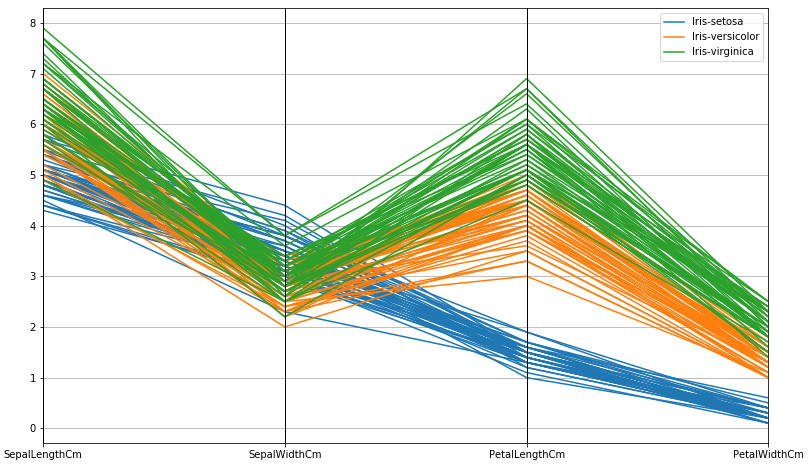
\includegraphics[width=0.7\textwidth]{iris-parallel.png}
 \caption{Parallel coordinates for the Iris dataset.}
 \label{fig:iris-parallel}
\end{figure}

\begin{figure}[ht]
 \centering
 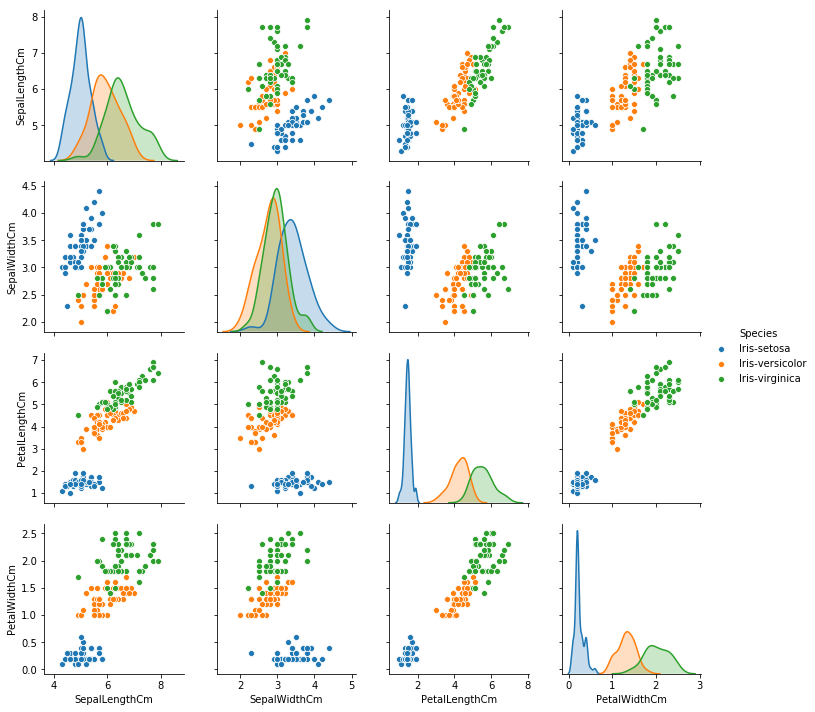
\includegraphics[width=0.9\textwidth]{iris-scatterplot.png}
 \caption{Scatter plot matrix for the Iris dataset.}
 \label{fig:iris-scatterplot}
\end{figure}

In the real-world, there are larger and more complex datasets than the Iris having hundreds of attributes and thousands or millions of items. For most of these cases, using the previous idioms is ineffective given the user cognition constraints for retaining many details, even when they are all shown at the same time, in addition to the screen size constraint. Next subsections describe two datasets considered relevant for this study and a possible exploratory analysis path supported by ML DR and Clustering algorithms.

\subsection{The FIFA 19 Complete Player Dataset}
\label{subsection1.1.1}

The FIFA dataset is currently one of the most popular datasets in Kaggle\footnote{https://www.kaggle.com/datasets (accessed on April 21th, 2019)}. It contains more than 18.000 player records of the popular video game, information representing the real state of players belonging to a wide variety of soccer clubs around the world. For each player there are 89 categorical and ordered attributes including age, nationality, overall scoring, potential, club, value, wage, preferred foot, international reputation, weak foot, skill moves, work rate, among many others. A possible user task could be to identify players with similar physical and game attributes to subsequently determine, for instance, the best conditions for training, trading options and match planning.

Figure \ref{fig:fifa-navio} summarizes this dataset by using Navio \cite{Guerra-Gomez2018Navio:Datasets} which is an interactive tool for exploring and navigating larger and high-dimensional datasets. More details about Navio are given in Section \ref{section4.3}. This is a good starting point for data understanding, nevertheless, it is not enough for fulfilling with the user task previously stated where attributes need to be aggregated in order to transversely identify similar players. 

\begin{figure}[ht]
 \centering
 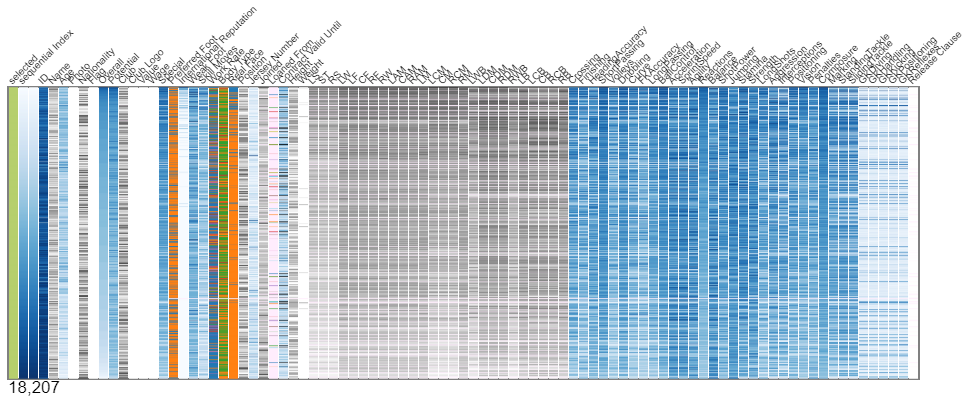
\includegraphics[width=0.9\textwidth]{fifa-navio.png}
 \caption{Visualization of the FIFA dataset in Navio.}
 \label{fig:fifa-navio}
\end{figure}

In this scenario is where ML can be useful. After validate data quality and transform attributes, a DR model is trained, for instance t-SNE, for producing an embedding that enables the identification of clusters of similar players. In addition, the position categorical attribute is used to encode the color in the embedding. The result is shown in Figure \ref{fig:fifa-tsne}. From this perspective, some analysis questions can be asked:

\begin{itemize}
\item Do clusters visually identified match with the position of the player? Do this match with other attribute in the dataset?
\item What characterize the players of the upper-left cluster and difference them from the players in the central cluster?
\item If goalkeepers (orange cluster) are excluded from the analysis, does the new t-SNE model produce the same three remaining clusters?
\item If physical attributes like height and weight are also excluded, is the player distribution in the embedding affected?  
\end{itemize}

\begin{figure}[ht]
 \centering
 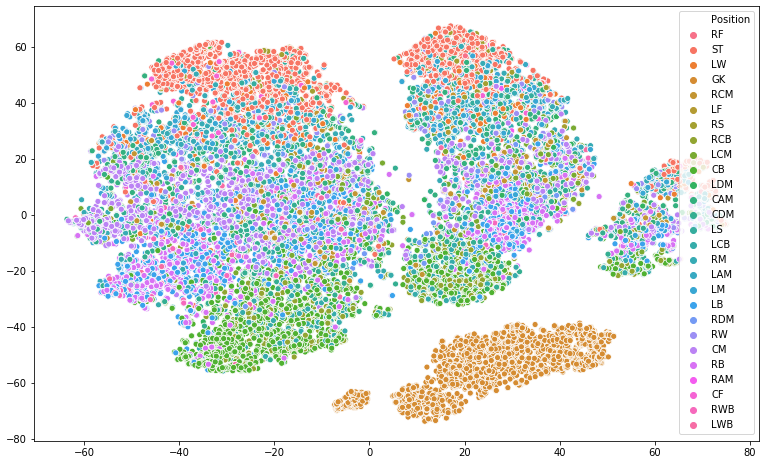
\includegraphics[width=0.7\textwidth]{fifa-tsne.png}
 \caption{DR embedding for the FIFA dataset using the t-SNE algorithm.}
 \label{fig:fifa-tsne}
\end{figure}

The first question could have a positive answer by performing model selection, which is addressed in Section \ref{section3.1}. Subsequent questions can be asked by additional experimentation where dataset is filtered or reduced and additional models are retrained in a iterative way. It is also required to be able for analyzing items in specific regions of the embedding. If the user is a ML-expert, they will not have problems to perform these analysis in the framework of their preference, otherwise, a tool for interact and interpret the model space and results is valuable. Some state of the art proposals are analyzed in Section \ref{section3.3}. Chapter \ref{chapter4} is focused on describing an improved proposal of a web interactive tool for answering these kind of EDA but also ML questions.

\subsection{The SALURBAL Dataset}
\label{subsection1.1.2}

SALURBAL is a five-year project aimed to study how urban environments and urban policies impact the health of city residents throughout Latin America \footnote{https://drexel.edu/lac/salurbal/overview/ (accessed on April 22th, 2019)}. For this purpose, datasets of Latin American cities and sub-cities containing urban form, landscape, street design and transportation metrics has been collected to subsequently determine which patterns emerge as mechanism for supporting the decision-making by domain-experts in fields like transportation and urban health. The sub-cities dataset has 1.438 items and 83 attributes, where all attributes are sequential except for name of the sub-city, type, city, country, presence of BRT, subway and aerial tram being categorical. Patterns can be builded as clusters, where sub-cities in the same cluster have similar metrics. In this sense, public policies already successful in one sub-city could have high probability to have success in other sub-city belonging to the same cluster. 

Again, the Figure \ref{fig:salurbal-navio} summarizes this dataset by using Navio enabling user to derive important instances by sorting and filtering interactions as explained in  in Section \ref{section4.3}.

\begin{figure}[ht]
 \centering
 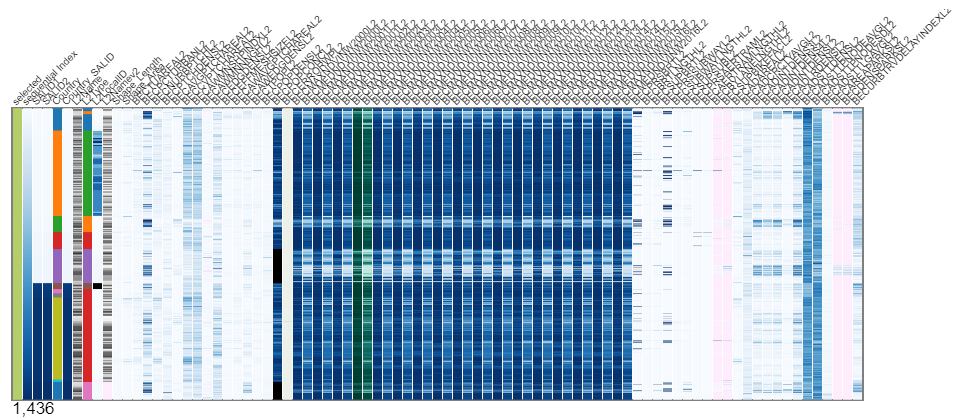
\includegraphics[width=0.9\textwidth]{salurbal-navio.png}
 \caption{Visualization of the SALURBAL dataset in Navio.}
 \label{fig:salurbal-navio}
\end{figure}

After validate data quality and transform attributes, a K-Means model is trained for producing groups of similar sub-cities that can be analyzed more easily. The model produces a cluster membership for each instance and a set of centroids but not much explanations about how these have been built. An alternative for gaining understanding is to observe the distribution of the original-space attributes, but since there are many of them, using t-SNE for visualizing the cluster distribution and validating their separability or overlapping is a reasonable choice. The result is shown in Figure \ref{fig:salurbal-kmeans-tsne}. Nevertheless, similar to the FIFA dataset, important questions need to be addressed: 

% Enfocar más a negocio
\begin{itemize}
\item Do the clusters of similar sub-cities match with the 2-dimensional distribution from the DR embedding?
\item What characterize the sub-cities of the blue cluster and difference them from the sub-cities in the red cluster?
\item Why the green cluster have only two sub-cities? Do they correspond to outliers having to be removed for the analysis? Does 4 clusters not represent a convenient data grouping?
\item These models are obtained including all sub-cities metrics for training. Would more make sense if models for Clustering and DR are trained by groups of attributes like urban landscape and street design?
\end{itemize}

\begin{figure}[ht]
 \centering
 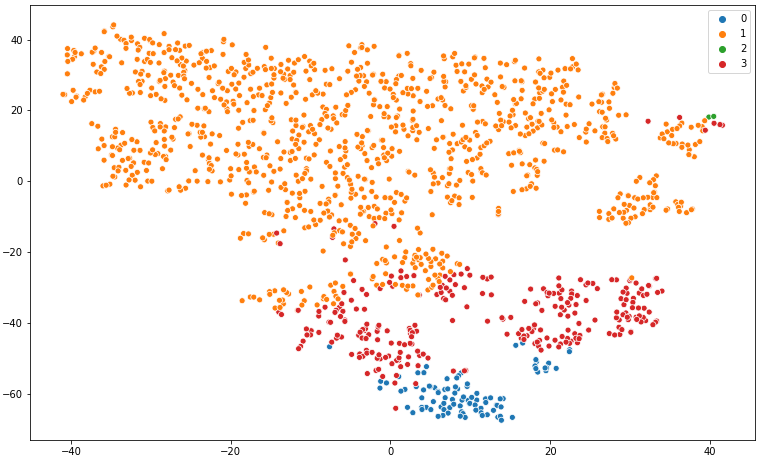
\includegraphics[width=0.7\textwidth]{salurbal-kmeans-tsne.png}
 \caption{DR embedding + Clustering for the SALURBAL dataset using the t-SNE and K-Means algorithms.}
 \label{fig:salurbal-kmeans-tsne}
\end{figure}

As stated in previous subsection, Chapters \ref{chapter3} and \ref{chapter4} are focused on describing some state of the art tools and an improved proposal of web interactive tool for answering these questions. 

\section{Document Structure} %Section - 1.2 
\label{section1.2}

This document is organized as follows: Chapter \ref{chapter2} shows the state of the art analysis for the Interactive ML and Interpretable ML sub-fields and the first contribution in terms of a set of guidelines for designing better and more user-centric ML systems. Chapter \ref{chapter3} describes some traditional DR and Clustering algorithms from a practical perspective and discuss the current advances for interact and interpret them in VA contexts. Chapter \ref{chapter4} presents the web interactive tool for exploring high-dimensional tabular data supported by t-SNE and K-Means. Chapter \ref{chapter5} evidences the results of the tool evaluation based on two real-world case studies. Finally, Chapter \ref{chapter6} concludes the work and presents the challenges and opportunities for the future.

\chapter{Designing User-Centric ML Systems}
\label{chapter2}

\graphicspath{{Chapter2/figs/}}

This chapter focuses on describing some advances in the context of Interactive ML and Interpretable ML. In first instance, both sub-fields are tackled independently but, in Section \ref{section2.3}, a discussion is stated in terms of how they can be combined for designing better and more user-centric ML systems. Finally, some related proposals in the context of DR and Clustering are presented in Section \ref{section2.4}.

\section{Interactive ML}
\label{section2.1}

The Human-Computer Interaction (HCI) field cares about human perception, cognition, intelligence, decision-making and interactive techniques of visualization. By the other hand, in Knowledge Discovery in Databases (KDD) automatic computational methods for finding previously unknown relationships in data are developed \cite{Holzinger2013}. By merging these fields, many research opportunities emerge including the paradigm where algorithms can interact with humans and optimize their learning behavior through these interactions \cite{Holzinger2016}. 

As described in \cite{Fails2003}, classic ML generally has some assumptions which can be addressed through the use of Interactive ML, such as:

\begin{itemize}
\item The introduction of many attributes in the model can become noise and therefore affect its performance. An Interactive ML system should provide to user the ability to perform attribute selection through a friendly interface.
\item When there is not enough training data, user also should be able to perform labeling under consideration or by a systematic way.
\item The system must quickly adapt after any user interaction affecting the data or model behavior. A delayed adaptation implies losing the user's attention.
\end{itemize}

More formally, Interactive ML is a co-adaptive process, driven by the user, but inherently dynamic in nature as the model and user evolve together during training \cite{Dudley2018}. These kind of systems should include interaction elements: \textbf{sample review}, \textbf{feedback assignment}, \textbf{model inspection} and \textbf{task overview}. By the other hand, an interface for Interactive ML should meet the following requirements: train very quickly, accommodate hundreds to thousands of features, perform feature selection and support tens to hundreds of thousands of training examples \cite{Fails2003}. A synthesis of a Interactive ML system is shown in Figure \ref{fig:InteractiveML} describing the direction of the interaction for each element. 

\begin{figure}[ht]
 \centering
 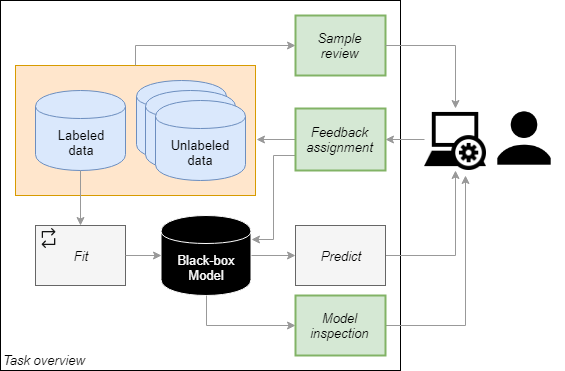
\includegraphics[width=0.7\textwidth]{InteractiveML.png}
 \caption{Block diagram representing an Interactive ML system.}
 \label{fig:InteractiveML}
\end{figure}

Known strategies for implementing the first two elements are briefly described in Subsections \ref{subsection2.1.1} and \ref{subsection2.1.2}. Although the \textbf{model inspection} element apparently does not have the same level of development, some relevant works are presented in Subsection \ref{subsection2.1.3}. For \textbf{task overview}, no one relevant work was found in the context of Interactive ML because this interface element is closely related to the specific knowledge domain. Model accuracy and related metrics are not enough to evaluate the task fulfillment, so this interface element should provide visibility of global objectives but also contextualize about other information such as availability of training data \cite{Dudley2018}.

Next subsections describe some related concepts to tackle the Interactive ML design process including some implementation scenarios.

\subsection{Dimensionality Reduction (DR)}
\label{subsection2.1.1}

In general terms, DR deals with the problem of finding meaningful low-dimensional structures (compact representation) from high-dimensional data \cite{Tenenbaum2000},\cite{Roweis2000}. For \textbf{sample review}, this is a valuable technique for representing high-dimensional data in principally two dimensions to validate the data distribution. Some algorithms for DR are Principal Component Analysis (PCA) \cite{PCA}, Self-Organized Maps (SOM) \cite{Kohonen1982Self-organizedMaps}, Isometric Mapping (ISOMAP) \cite{Tenenbaum2000}, t-Stochastic Neighborhood Embedding (t-SNE) \cite{VanDerMaaten2008}, and Uniform Manifold Approximation and Projection (UMAP) \cite{McInnes2018}. In general terms, many of the algorithms require a distance function (e.g. Euclidean distance) as method for calculating the similarity between pairs of instances \cite{Wenskovitch2018}, have their own training mechanism, may be sensible to random initialization at different levels and the selection of the hyper-parameters could satisfy diverse user intentions according to the domain of the problem.

PCA is a linear transformation algorithm that produce new uncorrelated dimensions (principal components) looking to maximize the variability represented in the dataset. SOM comes from the family of neural networks and use competitive learning to build a discrete representation of the data. ISOMAP is one of the first algorithms based on manifold learning and produces a low-dimensional embedding maintaining the geodesic distance between all instances causing preservation of global structures. Unlike ISOMAP, t-SNE retains particularly local structure but also some of global structure of the data. In many scenarios, t-SNE enables more the visual identification of clusters in comparison with ISOMAP but have the disadvantage of being expensive in  memory and processing and producing different embeddings with random initializations. UMAP is the newest technique and can compete with t-SNE for visualization but with superior run time performance.

DR can be used to achieve cluster-oriented task sequences such as verify clusters, name clusters and match cluster and classes \cite{Brehmer2014VisualizingSequences}. In this sense, DR and Clustering algorithms have been successfully combined for assist analysts in performing this kind of user tasks \cite{Wenskovitch2018}. Nevertheless, many challenges and opportunities need to be addressed. In addition, it is important to note that DR and Clustering algorithms are not only relevant for providing \textbf{sample review} as stated in \cite{Wenskovitch2017}, where a \textbf{feedback assignment} mechanism based on observation-level interaction is enabled for improving the cluster computation in an iterative way. 

\subsection{Active Learning and Visual Interactive Labeling}
\label{subsection2.1.2}

One way for achieving \textbf{feedback assignment} is by providing users the ability of labeling data. Active Learning (AL) consists of a series of analytical methods to select unlabeled data and present it to users in the form of queries for label assignment \cite{Holzinger2016}. Independently of the querying method used, the success of incorporating AL into an Interactive ML system lies on keeping the user labeling effort to a minimum. This can be achieved by only asking for feedback when the hope for a performance improvement given a specific query is high \cite{Olsson2009},\cite{Tong2001}.

Visual Interactive Labeling (VIL), in contrast to AL, delivers to user the selection of data candidates to be labeled. Nevertheless, user cognitive load can be reduced by incorporating visual techniques such as 2D colormaps, class coloring, convex hulls and butterfly plots \cite{Bernard2018b}. AL and VIL are used in scenarios where there is small amount of labeled data, and where the domain knowledge from users can be useful to improve unreliable predictions. 

In \cite{Bernard2018b}, authors present a comparison among multiple VIL and AL strategies. The decision regarding to use either of the two methods depends highly on the user task complexity, the \textbf{sample review} technique and the class separability. In general terms, both techniques can compete to produce better and faster classification models.

\subsection{Parameter Tuning and Error Discovery}
\label{subsection2.1.3}

Two useful strategies for \textbf{feedback assignment} and \textbf{model inspection} to be included into an Interactive ML system are parameter tuning and error discovery. 

% Parameter tuning
For the first strategy, the adjustment of model parameters does not imply necessarily, for instance, to provide the ability to modify the number of hidden layers or link weights, as in the context of neural networks. The goal is to design interaction mechanisms usable for users even when these are not experts in ML. In other words, putting model parameters in terms of the task domain, being this a non-trivial design decision. An example is shown in \cite{Kapoor2010}, where users are able to refine the parameters of the confusion matrix according to their preferences and thus re-train the model in an iterative way. For clustering, user actions affecting implicitly the model parameters include dragging points to form one or more new clusters, dragging an outlier into existing cluster, maximize one dimension weight and drag multiple sliders to equally large weights \cite{Self2016}. 

% error discovery
An example of Interactive ML system for error discovery is presented in \cite{Chen2018b}. From a website classification problem, domain knowledge about the target class is introduced facilitating error discovery through semantic data exploration. While elements such as \textbf{sample review} and \textbf{model inspection} are introduced, an eventual desire of Interactive ML systems is missing: the ability to perform labeling correction and re-train the model to evaluate if performance improves.

% Learning by user knowledge
It is also important to highlight some works focused on implement systems that learn explicitly from user knowledge and not refining an specific algorithm proposed in literature. In \cite{Brown2012}, users are able to build the distance function for two dimensions data projection according to their own sense of distance. In SIRIUS \cite{Dowling2018SIRIUS:Reductions}, coordinated dragging of instances and attributes in 2D panels offer a visual intuition about similarity-based relationships between them. In addition, a tool for clustering steered by user, having significantly higher quality than those from a pure algorithmic process, in proposed in \cite{Chang2016}.

\section{Interpretable ML}
\label{section2.2}

Interpretability is defined as the ability to explain or to present in understandable terms to a human \cite{Doshi-Velez2017c}. This definition by itself leaves more questions open than it solves and the decision behind delivering ML interpretability to users must be careful studied. Figure \ref{fig:interpretableML}, presents a condensed synthesis regarding to design aspects for delivering interpretability which are highly related to context, users, data and models \cite{Hohman2018},\cite{Doshi-Velez2017c},\cite{Lipton2017}. These aspects are grouped in six questions to be asked during the design process:

\begin{itemize}
    \item Why do you need to produce interpretability? Should the system be in the ability to generate trust about predictions? Does it protect sensitive information in the data?
    \item Who is the user of the system? Is the user a ML or a domain-expert?
    \item What are the most important elements of the data or the model to visualize?
    \item How do you plan to represent those most important elements? Is it important for user to interact with those elements?
    \item When generate interpretations? Is the model under continuous refinement  or was the model previously trained and validated?
    \item Where will the system be deployed? Is the system intended to support a real-world problem in a company? Does the system contribute to produce scientific advances in a specific ML sub-field or any other knowledge domain?  
\end{itemize}

\begin{figure}[ht]
 \centering
 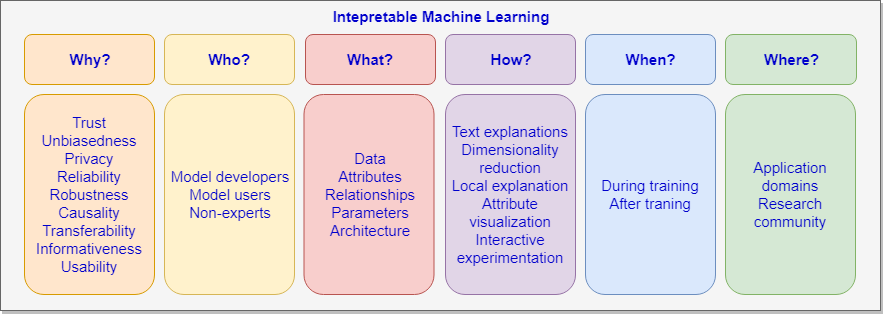
\includegraphics[width=0.9\textwidth]{InterpretableML.png}
 \caption{Aspects to consider when designing Interpretable ML systems.}
 \label{fig:interpretableML}
\end{figure}

Delivering interpretability implies opening the black-box and sometimes it could not be necessary and appropriate to do it, principally when there are no significant consequences for unacceptable results or the problem is sufficiently well-studied and validated in real applications that user trust the system’s decision, even if this is not perfect \cite{Doshi-Velez2017c}.

An example of interpretability in the DR context is DimReader \cite{Faust2019DimReader:Projections}. Building new axes representing infinitesimal perturbations in the embedding, this technique can be used to determine the regions where instances with similar range of values for a particular attribute are concentrated and the direction of the change.     

\subsection{Frameworks for Interpretability}

Some relatively basic techniques for interpret ML models are \cite{Becker2018MachineExplainability}: Permutation importance, for determining which attribute produces the highest performance decrease, and Partial dependence plots, for visualizing influence direction and shape when varying an attribute value.

A more sophisticated technique is LIME \cite{Ribeiro2016}, Local Interpretable Model-Agnostic Explanations, where a specific prediction is explained by learning an interpretable model locally. The result of LIME is a probability for each attribute value of belonging to the prediction class. In addition, the authors show the potential of the framework in applications based on tabular, image and text data. LIME is extended by SHAP \cite{Lundberg2017APredictions}, including an additional component based on the identification of a new class of additive attribute importance measures. LIME is also extended in \cite{Teso2018} and \cite{Phillips2018InterpretableLearning} to explain the query produced in an AL scenario. Local explanations are the base of works focused on produce global interpretation as proposed in \cite{Yang2018}. From contribution matrix representing the attribute importance for every data item, a binary tree is learned to explicitly represent the most important decision rules that are implicitly contained in the black-box model. 

Black-box Deep Learning models have the disadvantage of being the least interpretable because their large number of parameters as measure of complexity. Contributions in this field have been achieved by producing interpretation of the features learned at each layer of a Neural Network \cite{Yosinski2015a},\cite{Olah2018}. A more extensive literature review about interpretability in Deep Learning can be found in \cite{Zhang2018}.

\section{The Link Between Both Worlds}
\label{section2.3}

Interactive ML and Interpretable ML in the most of cases previously described has been tackled as isolated concepts. In some scenarios, mechanisms for \textbf{sample review} and \textbf{feedback assignment} (e.g. labeling or parameter tuning) may not be enough to successfully fulfill the user task. \textbf{Model inspection} implies opening the black-box and presenting it to user in an interpretable way and model interpretation indicates the ability to provide explanations about their inner working which could help users to better understand their results \cite{Doshi-Velez2017c}. This extension could support the \textbf{task overview} interface element because, as stated in \cite{Doshi-Velez2017c}, \cite{Lipton2017}, model interpretation is used to achieve other important requirements in user-centric ML systems such as trust, unbiasedness, privacy, reliability, robustness, causality, transferability, informativeness and usability.

In other words, \textbf{an Interactive ML system is not necessarily interpretable in terms of what model is learning and, in the opposite case, an Interpretable ML system could not involve all enough elements of interaction to perform the task in an usable and efficient way}. Designers must not forget the system is constrained by an user task and users are the ones who have the power to determine if the task is effectively fulfilled. User evaluation for interactivity and interpretability, as in any HCI study, must be considered.

%After establishing the bases for designing user-centric ML systems, some DR and Clustering algorithms are presented from a practical perspective. This chapter is not focused in determining the best algorithm for reducing or clustering data but discussing about how these behave for some real-world datasets. The third section of this chapter concentrates in summarize some tools that use this kind of algorithms while user can interact and interpret them.

%Figure \ref{fig:dr-matrix} shows some experiments performed for 4 datasets with different level of complexities using 4 of the DR algorithms previously described: the Iris dataset, the Breast Cancer dataset, the FIFA dataset and the SALURBAL dataset. A class attribute is used for color encoding: species, diagnosis, position and sub-city type, respectively. Hyper-parameter tuning is not considered, the most important aspect to evaluate is the ability of the algorithms to build embeddings with visually identifiable clusters. For the first dataset, all algorithms seem to work similar separating one of the three classes and reflecting no linear separability of the remaining classes.

%\begin{figure}[ht]
% \centering
% \includegraphics[width=1.0\textwidth]{DRmatrix.png}
% \caption{DR embeddings for 4 datasets: the Iris dataset, the Breast Cancer dataset, the FIFA dataset and the SALURBAL dataset.}
% \label{fig:dr-matrix}
%\end{figure}

%As appreciate, PCA and ISOMAP tend to overlap the classes making difficult for user to   

%\section{Clustering Data}
%\label{section2.5}

%K-Means
%Spectral
%Agglomerative
%DBSCAN

\section{EDA Tools for Interacting and Interpreting DR and Clustering}
\label{section2.4}

Many researchers have proposed to integrate ML in systems or tools for analyzing data. In \cite{Endert2017b}, a wide range of works are presented and some challenges and opportunities are presented including: (1) incorporation of user feedback, (2) balance human and machine efforts, responsibility and tasks, (3) control of system complexity, (4) visualization of intermediate results, and (5) interpretability. In the context of DR and Clustering, \cite{Wenskovitch2018} and \cite{Sacha2017g} derive from literature review the user tasks and interaction mechanisms incorporated in this kind of systems:

\begin{itemize}
\item DR: See distribution of instances, identify clusters, rotate the embedding, reposition instances, measure distances between instances, change distance metric, select different attributes, modify the weight of an attribute, obtain attribute values and select the algorithm and modify its hyper-parameters.
\item Clustering: Determine cluster structure, label / annotate clusters, merge or split clusters, reposition instances, select different attributes, modify the weight of an attribute, obtain attribute values and select the algorithm and modify its hyper-parameters.
\end{itemize}

To the best of our knowledge, a first effort of interactive tool for DR and Clustering is Divvy \cite{Lewis2013Divvy:Analysis}. In Divvy, user is able to load a dataset and evidence its shape, train some DR and Clustering models changing the hyper-parameters and visualize the results in multiple embeddings. In this standalone tool, no other interaction mechanism is considered. Embedding Projector \cite{Smilkov2016EmbeddingEmbeddings} is a web tool from the Tensorflow \cite{Abadi2016TensorFlow:Learning} ecosystem and it enables additional interactions for embeddings including zooming, rotation, panning, query for getting attribute values and nearest-neighbors. Three DR algorithms are implemented in Embedding Projector (PCA, t-SNE and a linear projection of any two custom vectors) but experimentation is limited to 5 pre-loaded datasets. A-tSNE \cite{Pezzotti2016ApproximatedAnalytics} is a complementary tool mainly focused on fast execution of the t-SNE algorithm for progressive analytics. In a first stage, the tool builds an approximated embedding to subsequently refine the approximation in areas of interest for the user. Figure \ref{fig:interactiveDR} shows screenshoots of the works previously mentioned. Other improvement of t-SNE is proposed in \cite{Pezzotti2018LinearWeb}. In this case, Tensorflow.js \cite{Smilkov2019TensorFlow.js:Beyond} is extended with this DR algorithm for execution in the browser taking advantage of the tensor data structures and WebGL textures for fast execution.

\begin{figure}[ht]
 \centering
 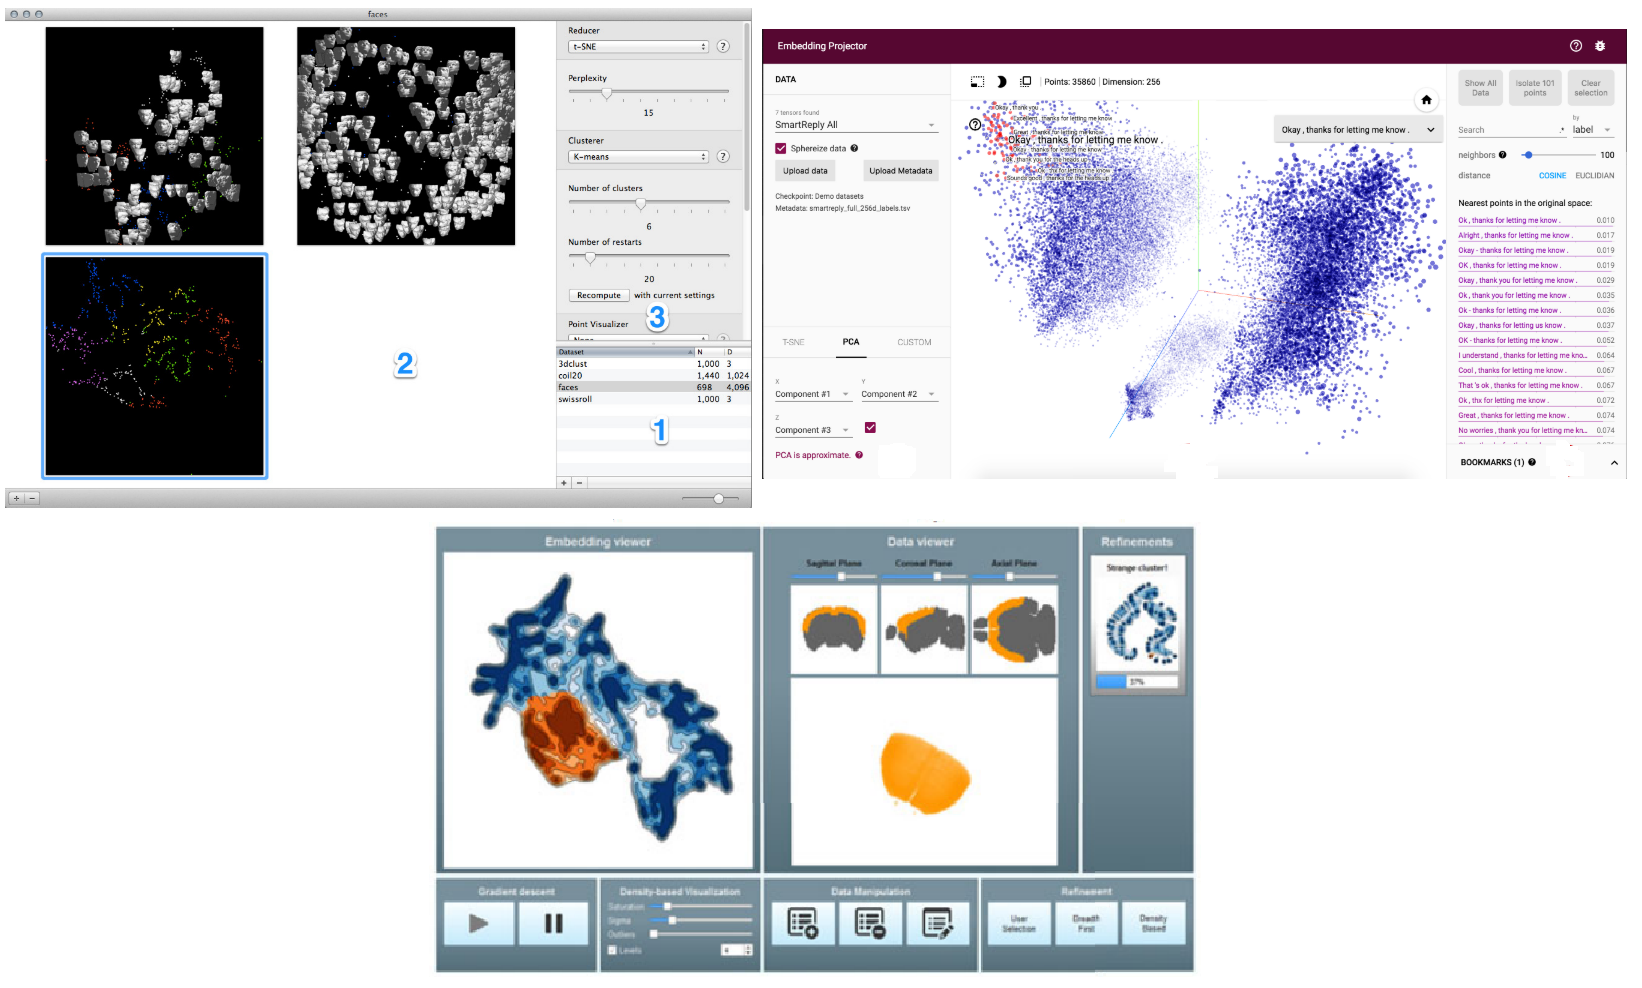
\includegraphics[width=0.9\textwidth]{InteractiveDR.png}
 \caption{Divvy \cite{Lewis2013Divvy:Analysis} (top left), Embedding Projector \cite{Smilkov2016EmbeddingEmbeddings} (top right) and A-tSNE \cite{Pezzotti2016ApproximatedAnalytics} (bottom) for interactive DR and Clustering.}
 \label{fig:interactiveDR}
\end{figure}

These proposals inspire the development of the tool explained in Chapter \ref{chapter3}. The main improvement with respect to these tools is the ability for domain-expert users to train DR and Clustering models for supporting clustering-oriented EDA tasks without losing the overall context of the data in the same interactive tool. This context of the data is also used as an initial mechanism for providing interpretability for the available models.


\chapter{MLExplore.js: A Web Interactive Tool for Exploring High-Dimensional Data}
\label{chapter3}

\graphicspath{{Chapter3/figs/}}

From Chapter \ref{chapter2}, 4 interface elements to be included in an Interactive ML system are stated and Interpretable ML is proposed as a mechanism for complementing the \textbf{model inspection} and \textbf{task overview} elements. This chapter also highlights some relevant works for interacting with and interpreting DR and Clustering models for data analysis. An important focus of the state of the art proposals in Interactive ML is to provide user with the ability for hyper-parameter exploration looking to produce a good representation of embeddings and clusters. The discussion about what is a good representation, being the general problem in unsupervised learning, continues open. In addition, researchers also focus on deriving the most relevant interaction elements for supporting the data exploration. These proposals can be complemented with components for data exploration and navigation, being this a mandatory stage in any data analytics process, and model results understanding in terms of attributes in the original space.  In this work, MLExplore.js, a web interactive tool more suitable for domain-experts users with cluster-oriented tasks sequences in high-dimensional data rather is presented. Figure \ref{fig:mlexplore-components} shows the components of the tool and the dotted lines represent interaction possibilities for the user. Each of these components are explained in the subsequent sections. 

\begin{figure}[ht]
 \centering
 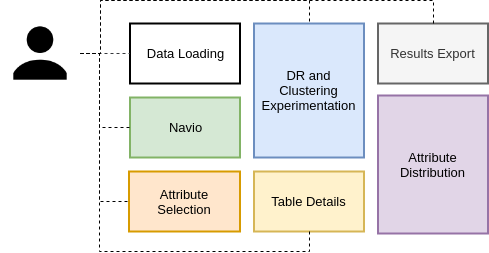
\includegraphics[width=0.7\textwidth]{MLExplore-components.png}
 \caption{MLExplore.js components and interaction possibilities for users.}
 \label{fig:mlexplore-components}
\end{figure}

In addition, the decision behind implementing the tool in a web-based environment with local ML computation using only JavaScript libraries for shareability, interactivity and on-device computation is inspired by Tensorflow.js \cite{Smilkov2019TensorFlow.js:Beyond}. These properties are important for domain-expert users because enable them to perform ML-based EDA without requiring complex infrastructure and easily share their work with colleagues and community in general. By the other hand, local computation also has the advantage of privacy preserving, because despite the tool is available on internet, the data remains in the browser. Currently, the ML community in JavaScript does not have the same level of development compared to other languages like Python and R, reason why alternatives for including ML algorithms in the tool are limited. Nevertheless, it is expected that this panorama continues evolving during the next years.

\section{Data Loading}
\label{section3.1}

In many cases, domain-expert users store data in local semi-structured files, principally when the size does not demand to invest resources to maintain TI infrastructures increasing the complexity of the project.
Currently. the tool supports loading datasets from a local path in CSV format and file size constraint depends on browser capabilities. In addition, as shown in Figure \ref{fig:load-dataset-component}, 4 low size datasets for trainees are available: (1) the Fisher's Iris \cite{FisherIris}, the Zoo dataset, the Breast Cancer dataset and the Heart Diseases dataset. All these datasets are available at UCI Machine Learning Repository \cite{Dua2017UCIRepository}.

\begin{figure}[ht]
 \centering
 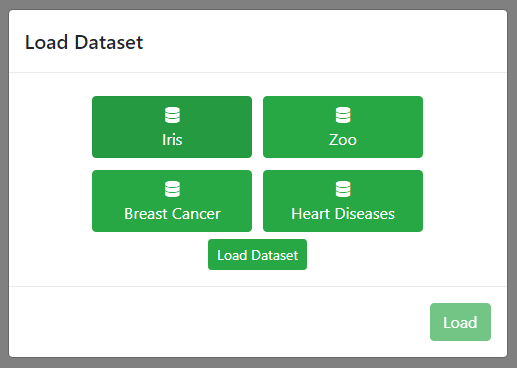
\includegraphics[width=0.5\textwidth]{load-dataset.png}
 \caption{Data Loading component.}
 \label{fig:load-dataset-component}
\end{figure}

\section{Data Exploration and Navigation (Navio)}
\label{section3.2}

The intention of using ML for exploring high-dimensional data does not imply that user should forget about descriptive techniques enabled also for gaining data understating. Distribution summarization, correlation analysis and outliers identification, among others, are generalized user tasks that always must be covered in any analytic process and considered in an Interactive ML tool as a element for \textbf{sample review}. Navio \cite{Guerra-Gomez2018Navio:Datasets} is an interactive web-based tool designed for achieving these kind of tasks but also for data navigation implementing three kinds of interactions: sorting, filtering a range and filtering by value. Because this tool is available as a JavaScript widget, the incorporation as a component requires a little effort and enables a more informed ML model usage. Figure \ref{fig:navio-component} shows the Navio component for the Breast Cancer dataset. 

\begin{figure}[ht]
 \centering
 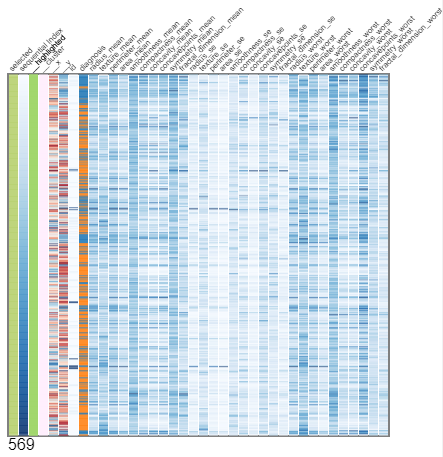
\includegraphics[width=0.5\textwidth]{navio.png}
 \caption{Data Exploration and Navigation (Navio) component.}
 \label{fig:navio-component}
\end{figure}

In addition, Navio component also includes three new attributes representing the results of the last trained models. This means, two new attributes for the embedding and other one for the clusters. In this way, user is enabled to extend the data exploration and navigation in the original space to, for instance, sort by embedding dimensions to discover correlations of them with data attributes or filter by a particular cluster. A fourth artificial attribute is used to retain highlighting actions performed by the user in the DR and Clustering Experimentation component.

\section{Attribute Selection}
\label{section3.3}

Attribute selection is an important stage in any ML process and it is a mechanism for providing \textbf{feedback assignment} when the domain-expert user decides if the presence of absence of a specific attribute can considerably affect the performance of a model. After the user load a dataset and performs an overview in Navio, all attributes are listed including an icon representing its type and a checkbox for attribute selection. Currently, the tool is able to identify two types of attributes: numerical and categorical. By default, all numerical attributes are selected meaning that these will be used for training the models. The reason behind this decision is related to the constraint of the models available in the tool for working only with numerical data. A Functionality for filter attributes by partial name matching, principally useful when there are a lot of similar attribute names, is also provided. Figure \ref{fig:attribute-selection-component} shows the Attribute Selection component for the Breast Cancer dataset.

\begin{figure}[ht]
 \centering
 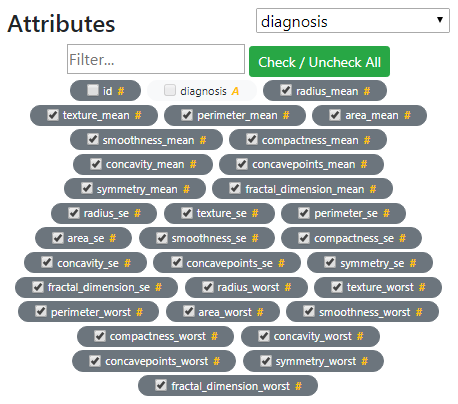
\includegraphics[width=0.5\textwidth]{attribute-selection.png}
 \caption{Attribute Selection component.}
 \label{fig:attribute-selection-component}
\end{figure}

In addition, the user can select the attribute for color encoding in the upper-right combobox affecting the DR and Clustering Experimentation and the Attribute Distribution components. If the attribute is categorical, a categorical color scheme is used but if the attribute is numerical, the color scheme selected by MLExplore.js is one sequential. Automatically, a categorical attribute with low cardinality is selected. A strategy for gaining interpretability about the results of the t-SNE algorithm is by selecting any numerical attribute and evidencing that higher values are concentrated in a zone of the embedding and lower values in a different. This principle is similar to the axis lines built in DimReader \cite{Faust2019DimReader:Projections} but not including additional elements which can make it more difficult to use these kind of tools.

\section{DR and Clustering Experimentation}
\label{section3.4}

The user is enabled to train in the browser two kind of DR and Clustering models for supporting the cluster-oriented EDA using the widely known t-SNE \cite{VanDerMaaten2008} and K-Means \cite{Lloyd1982LeastPCM} algorithms, and that currently have implementations in JavaScript \cite{Pezzotti2018LinearWeb},\cite{Asensio2018Ml-kmeans}. The result of t-SNE consist of two new dimensions or attributes being used for draw the a embedding (scatter plot) evidencing an overview of the data distribution. The result of K-Means is used for encode the color in the embedding and the Attribute Distribution component. For both models, the user can perform \textbf{feedback assignment} by modifying the hyper-parameters, re-train the models and visualize how the embedding and clusters changes in an iterative way. This is a way of \textbf{model inspection}. The t-SNE hyper-parameter ranges are based on \cite{Wattenberg2016HowEffectively}. Up to 10 number of clusters for K-Means training is allowed, this limit can be increased but losing readability because number of colors need to difference cluster or classes. MLExplore.js also enables user to scale attributes avoiding that models optimize paying more attention to attributes with high-range values. Figure \ref{fig:dr-and-clustering-experimentation-component} shows the DR and Clustering Experimentation component for the Breast Cancer dataset.

\begin{figure}[ht]
 \centering
 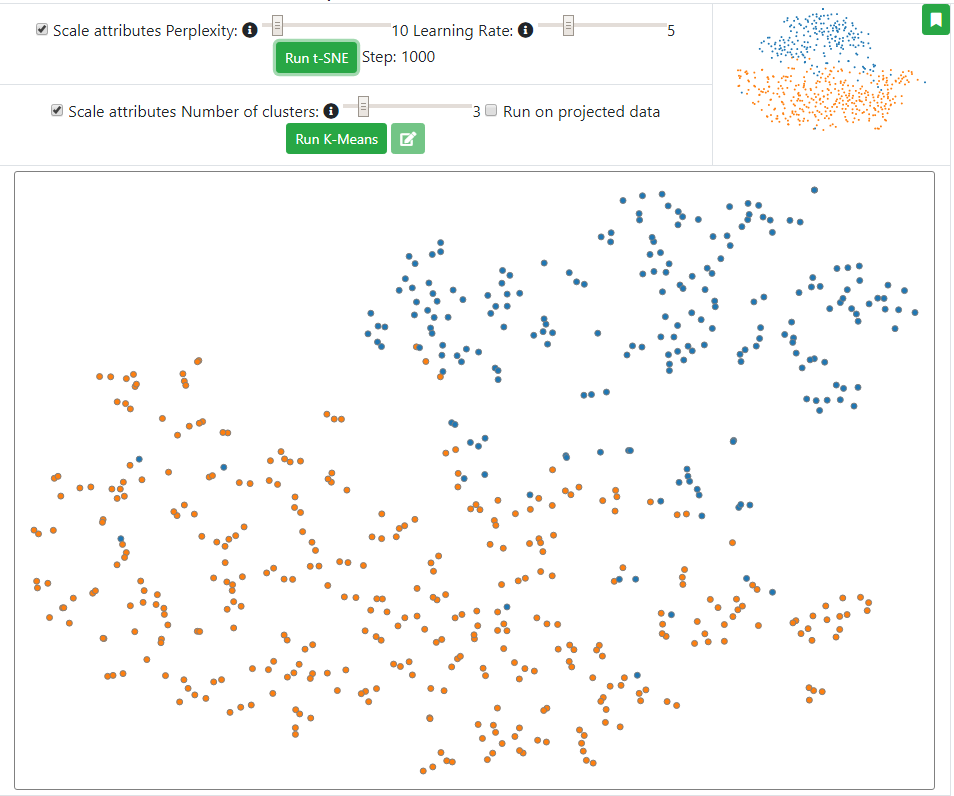
\includegraphics[width=0.7\textwidth]{dr-and-clustering-experimentation.png}
 \caption{DR and Clustering Experimentation component.}
 \label{fig:dr-and-clustering-experimentation-component}
\end{figure}

When finishing the training of a new model, additional changes to the embedding are produced: (1) Navio component is updated for including the results of the models, as explained in Section \ref{section3.2} and (2) Attribute Distribution component changes for evidencing the new clusters by color encoding. The user has the option to temporally save the current embedding and visualize the upper-right panel for model comparison. In addition, user is also enabled to change the cluster membership according to their judgment and highlight square regions of interest and visualize where some data instances are located in the Attribute Distribution component and how much their embedding distribution is differentiated from a previous experiment.

As a complementary \textbf{model inspection} strategy for interpretability, when user clicks a specific data instance, the embedding is updated to highlight the 20 nearest neighbors in terms of the Euclidean distance. This calculation can be useful to visually validate if, with those hyper-parameters, t-SNE is able to capture the similarity among data instances based in a more traditional metric that can be more easily understood by non-ML users. 

\section{Attribute Distribution}
\label{section3.5}

DR and Clustering models learn from similarity measures. If two data instances are close in the embedding or belongs to the same clusters, hopefully these instances will have similar attribute values. The purpose of this component is to evidence if this principle is fulfilled in a generalized way for \textbf{model inspection}, provide trust to user and advance in the insights extraction process. For each attribute used to train the models, a ticks chart or a scatter plot representing its distribution is displayed. The decision behind display a ticks chart or a scatter plot depends on the attribute currently used for color encoding. Figure \ref{fig:attribute-distribution-component} shows the Attribute Distribution component for the Breast Cancer dataset.

\begin{figure}[ht]
 \centering
 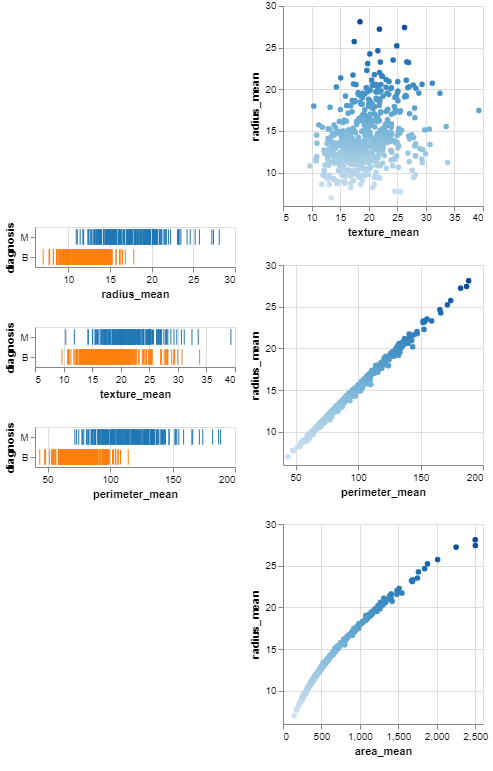
\includegraphics[width=0.4\textwidth]{attribute-distribution.png}
 \caption{Attribute Distribution component for categorical (left) and sequential (right) color encoding.}
 \label{fig:attribute-distribution-component}
\end{figure}

As mentioned before, this component is also affected by the DR and Clustering Experimentation component when user highlight a region of interest in the embedding. In the Attribute Distribution component, all data instances not included in the highlighting are opaqued. In this way, users are enabled to obtain details on demand.

\section{Table Details}
\label{section3.6}

Table Details component, a complementary \textbf{sample review} element, is included in MLExplore.js for enabling the data exploration in the most traditional way. This table is extended for searching data instances for by specific values, this functionality is useful in datasets like FIFA and SALURBAL in order to locate players, teams, positions or sub-cities, cities, countries, respectively. When user clicks a specific row, the embedding is updated to show the 20 nearest neighbors as previously explained in the DR and Clustering Experimentation component. Figure \ref{fig:table-details-component} shows this component for the Breast Cancer dataset.

\begin{figure}[ht]
 \centering
 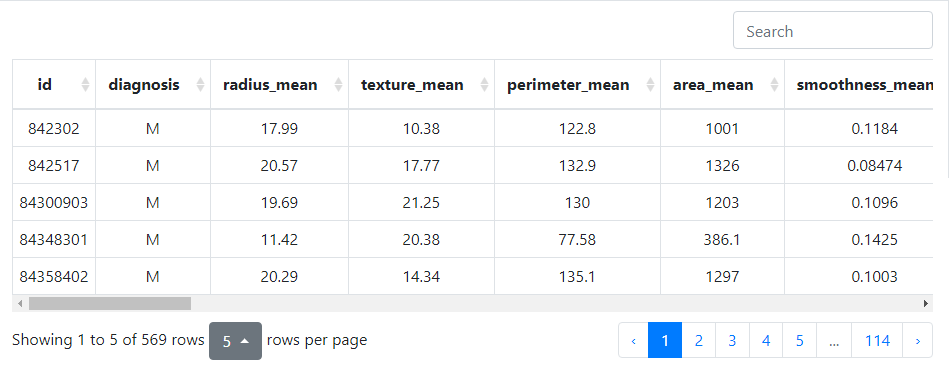
\includegraphics[width=0.9\textwidth]{table-details.png}
 \caption{Table Details component.}
 \label{fig:table-details-component}
\end{figure}

\section{Results Export}
\label{section3.7}

Finally, in any stage of the experimentation user is able to download the dataset in CSV format including all new artificial attributes (Navio selection, x-axis and y-axis embedding, clusters and highlighting) and a configuration file in JSON format. As shown in \ref{fig:results-export-component}, options provided when downloading the dataset include: download only model results, all attributes and model results and selected attributes and model results. The configuration file contains a list of the attributes, their identified type and which of these were used to train the models and encode the color during the last experimentation. Because the dataset is download in a widely known format, user can use it to continue with analysis process in almost any tool. Currently, this file only stores the hyper-parameters of the last trained models for the t-SNE and K-Means algorithms.

\begin{figure}[ht]
 \centering
 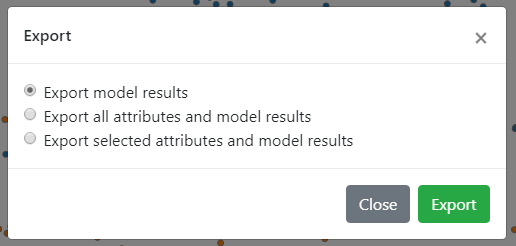
\includegraphics[width=0.5\textwidth]{results-export.png}
 \caption{Results Export component.}
 \label{fig:results-export-component}
\end{figure}
%!TEX root = ../thesis.tex
%*******************************************************************************
%****************************** Fourth Chapter **********************************
%*******************************************************************************
\chapter{A Web Interactive Tool for Exploring High-Dimensional Data}
\label{chapter4}

\graphicspath{{Chapter4/figs/}}

%% Cites required
One of the main focus of the state of the art proposals in Interactive ML is to provide user with the ability for model space exploration looking to produce a good representation of embeddings and clusters. The discussion about what is a good representation, being the general problem in unsupervised learning, continues open. In addition, researchers also focus on deriving the most relevant interaction elements for supporting the data exploration. These proposals can be complemented with components for data exploration and navigation, being this a mandatory stage in any data analytics study, and model results understanding in terms of attributes in the original space.  In this work, a web interactive tool more suitable for domain-experts users with cluster-oriented tasks in high-dimensional data rather than just interaction with DR and Clustering models is presented. Design decisions about components or functionalities provided by the tool are explained in the subsequent sections. 

In addition, the decision behind implementing the tool in a web-based environment with local ML computation using only JavaScript libraries for shareability, interactivity and on-device computation is inspired by \cite{Smilkov2019TensorFlow.js:Beyond}. These properties are important for domain-expert users because enable them to perform ML-based EDA without requiring complex infrastructure and easily share their work with colleagues and community in general. By the other hand, local computation also has the advantage of privacy preserving, because despite the tool is available on internet, the data remains in the browser. 

\section{Load Dataset}
\label{load-dataset-section}

In many cases, domain-expert users store data in local semi-structured files, principally when the size does not demand to invest resources to maintain TI infrastructures increasing the complexity of the project.
The tool supports loading datasets from a local path in CSV format and file size constraint depends on browser capabilities. In addition, as sown in Figure \ref{fig:load-dataset-component}, some low size datasets for trainees are available: (1) the Fisher's Iris \cite{FisherIris}, the Zoo dataset \cite{*}, the Breast Cancer dataset \cite{*} and the Heart Diseases dataset \cite{*}.

\begin{figure}[ht]
 \centering
 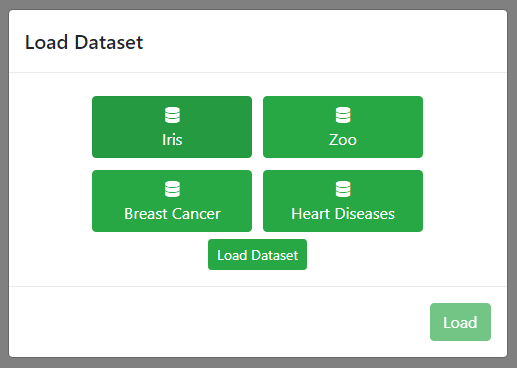
\includegraphics[width=0.5\textwidth]{load_dataset.png}
 \caption{Load Dataset component.}
 \label{fig:load-dataset-component}
\end{figure}

\section{Attribute Selection}
\label{attribute-selection-section}

Attribute selection is an important stage in any ML process. After the user load a dataset, all attributes are listed including an icon representing its type and a checkbox for attribute selection. Currently, the tool is able to identify three types of attributes: numerical, boolean and categorical or strings. Boolean type is automatically identified when the attribute has only two values: 0 and 1. By default, all numerical and boolean attributes are selected meaning that these will be used for training the models. The reason behind this decision is related to the constraint of the models available in the tool of working only with numerical data. Nevertheless, categorical attributes are available for color encoding representing classes or clusters. The user can select the attribute for color encoding in the upper-right combobox, the tool automatically selects a categorical attribute with low cardinality. Figure \ref{fig:attribute-selection-component} shows the Attribute Selection component for the FIFA dataset.

\begin{figure}[ht]
 \centering
 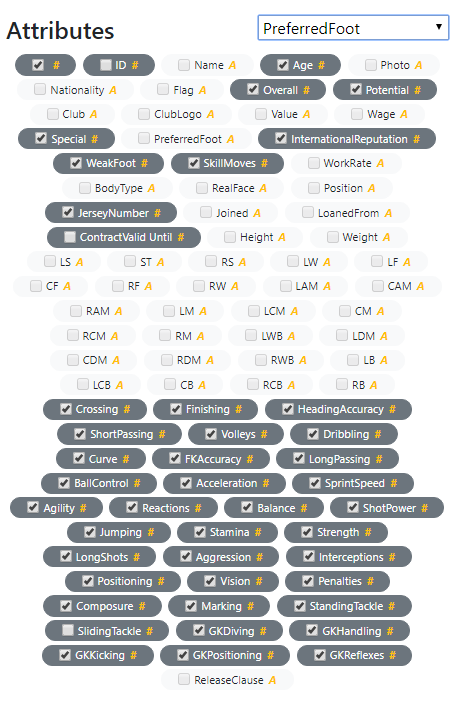
\includegraphics[width=0.5\textwidth]{attribute-selection.png}
 \caption{Attribute Selection component.}
 \label{fig:attribute-selection-component}
\end{figure}

\section{Data Exploration and Navigation (Navio)}
\label{navio-section}

The intention of using ML for exploring high-dimensional data does not imply that user should forget about descriptive techniques enabled also for gaining data understating. Distribution summarization, correlation analysis and outliers identification, among others, are generalized user tasks that always must be covered in any analytic process. Navio \cite{Guerra-Gomez2018Navio:Datasets} is an interactive web-based tool designed for achieving these kind of tasks but also for data navigation implementing three interactions: sorting, filtering a range and filtering by value. Because this tool is available as a JavaScript widget, the incorporation as a component complementary to attribute selection-level interactions looking for a more informed ML models usage is highly valuable for domain-expert users. Figure \ref{fig:navio-component} shows the Navio component for the FIFA dataset.  

\begin{figure}[ht]
 \centering
 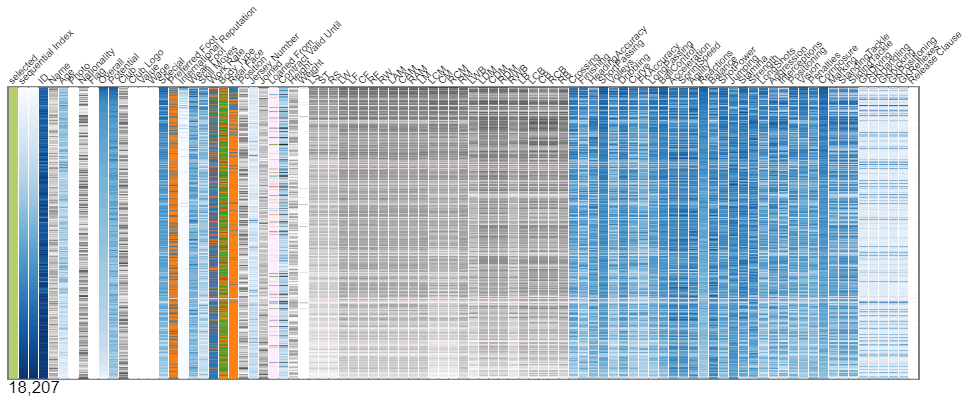
\includegraphics[width=0.9\textwidth]{navio.png}
 \caption{Data Exploration and Navigation (Navio) component.}
 \label{fig:navio-component}
\end{figure}

\section{Model Space Exploration}
\label{model-space-exploration-section}

The user is enabled to train in the browser two kind of models for supporting the cluster-oriented EDA: t-SNE \cite{VanDerMaaten2008} and K-Means \cite{Lloyd1982LeastPCM}. 

%In order to provide a mechanism to carry out cluster-oriented task sequences, as defined in \cite{*}, user can select a categorical attribute for color encoding, in the case of labeled data, but in general we provide an additional functionality to train a K-Means clustering model and use its results for color encoding.

%For both algorithms, t-SNE and K-Means, user is able to modify the model hyper-parameters and visualize how embedding is affected in an iterative way. 

\section{Results Understanding}
\label{results-understanding-section}

The last component is based on proposals for local interpretability like LIME \cite{Ribeiro2016} and extensions

%Because Inter2DR is a tool for domain-expert users, we decide to include two complementary groups of idioms to validate the embedding and clustering models by observation of independent attribute distributions and instance details in a table. These components present coordinate highlighting, enabling user to quickly compare instances in the embedded space with their attribute values in the original space and vice versa.

\section{Reproducing Experiments}
\label{results-understanding-section}

Finally, in any stage of the experimentation user is able to locally save and load a configuration file. This file contains a list of the attributes, their type and which of these were used to train the models and encode the color. Currently, the configuration file only stores the hyper-parameters and results of the last trained models for the t-SNE and K-Means algorithms. Another limitation of this component is related to storing the Navio state, meaning that the interaction sequence for sorting or filtering carried out during the previous experimentation cannot be reproduced. In other words, user is able to observe the results of a previous experiment and re-train the models using the same hyper-parameters for achieving comparable results only if the dataset was not filtered. 
%!TEX root = ../thesis.tex
%*******************************************************************************
%****************************** Fifth Chapter **********************************
%*******************************************************************************
\chapter{Case Studies}
\label{chapter5}

\graphicspath{{Chapter5/figs/}}

%********************************** %First Section  **************************************
\section{The FIFA case study} %Section - 5.1 
\label{section5.1}



%********************************** %Second Section  **************************************
\section{The SALURBAL case study} %Section - 5.2 
\label{section5.2}
%%!TEX root = ../thesis.tex
%*******************************************************************************
%****************************** Sixth Chapter **********************************
%*******************************************************************************
\chapter{Conclusions}
\label{chapter6}

Conclusions ...
%\include{Chapter7/chapter7}



% ********************************** Back Matter *******************************
% Backmatter should be commented out, if you are using appendices after References
%\backmatter

% ********************************** Bibliography ******************************
\begin{spacing}{0.9}

% To use the conventional natbib style referencing
% Bibliography style previews: http://nodonn.tipido.net/bibstyle.php
% Reference styles: http://sites.stat.psu.edu/~surajit/present/bib.htm

\bibliographystyle{apalike}
%\bibliographystyle{unsrt} % Use for unsorted references  
%\bibliographystyle{plainnat} % use this to have URLs listed in References
\cleardoublepage
\bibliography{References/mendeley} % Path to your References.bib file


% If you would like to use BibLaTeX for your references, pass `custombib' as
% an option in the document class. The location of 'reference.bib' should be
% specified in the preamble.tex file in the custombib section.
% Comment out the lines related to natbib above and uncomment the following line.

%\printbibliography[heading=bibintoc, title={References}]


\end{spacing}

% ********************************** Appendices ********************************

%\begin{appendices} % Using appendices environment for more functunality

%%!TEX root = ../thesis.tex
% ******************************* Thesis Appendix A ****************************
\chapter{How to install \LaTeX} 

\section*{Windows OS}

\subsection*{TeXLive package - full version}
\begin{enumerate}
\item	Download the TeXLive ISO (2.2GB) from\\
\href{https://www.tug.org/texlive/}{https://www.tug.org/texlive/}
\item	Download WinCDEmu (if you don't have a virtual drive) from \\
\href{http://wincdemu.sysprogs.org/download/}
{http://wincdemu.sysprogs.org/download/}
\item	To install Windows CD Emulator follow the instructions at\\
\href{http://wincdemu.sysprogs.org/tutorials/install/}
{http://wincdemu.sysprogs.org/tutorials/install/}
\item	Right click the iso and mount it using the WinCDEmu as shown in \\
\href{http://wincdemu.sysprogs.org/tutorials/mount/}{
http://wincdemu.sysprogs.org/tutorials/mount/}
\item	Open your virtual drive and run setup.pl
\end{enumerate}

or

\subsection*{Basic MikTeX - \TeX~ distribution}
\begin{enumerate}
\item	Download Basic-MiK\TeX (32bit or 64bit) from\\
\href{http://miktex.org/download}{http://miktex.org/download}
\item	Run the installer 
\item	To add a new package go to Start >> All Programs >> MikTex >> Maintenance (Admin) and choose Package Manager
\item	Select or search for packages to install
\end{enumerate}

\subsection*{TexStudio - \TeX~ editor}
\begin{enumerate}
\item	Download TexStudio from\\
\href{http://texstudio.sourceforge.net/\#downloads}
{http://texstudio.sourceforge.net/\#downloads} 
\item	Run the installer
\end{enumerate}

\section*{Mac OS X}
\subsection*{MacTeX - \TeX~ distribution}
\begin{enumerate}
\item	Download the file from\\
\href{https://www.tug.org/mactex/}{https://www.tug.org/mactex/}
\item	Extract and double click to run the installer. It does the entire configuration, sit back and relax.
\end{enumerate}

\subsection*{TexStudio - \TeX~ editor}
\begin{enumerate}
\item	Download TexStudio from\\
\href{http://texstudio.sourceforge.net/\#downloads}
{http://texstudio.sourceforge.net/\#downloads} 
\item	Extract and Start
\end{enumerate}


\section*{Unix/Linux}
\subsection*{TeXLive - \TeX~ distribution}
\subsubsection*{Getting the distribution:}
\begin{enumerate}
\item	TexLive can be downloaded from\\
\href{http://www.tug.org/texlive/acquire-netinstall.html}
{http://www.tug.org/texlive/acquire-netinstall.html}.
\item	TexLive is provided by most operating system you can use (rpm,apt-get or yum) to get TexLive distributions
\end{enumerate}

\subsubsection*{Installation}
\begin{enumerate}
\item	Mount the ISO file in the mnt directory
\begin{verbatim}
mount -t iso9660 -o ro,loop,noauto /your/texlive####.iso /mnt
\end{verbatim}

\item	Install wget on your OS (use rpm, apt-get or yum install)
\item	Run the installer script install-tl.
\begin{verbatim}
	cd /your/download/directory
	./install-tl
\end{verbatim}
\item	Enter command `i' for installation

\item	Post-Installation configuration:\\
\href{http://www.tug.org/texlive/doc/texlive-en/texlive-en.html\#x1-320003.4.1}
{http://www.tug.org/texlive/doc/texlive-en/texlive-en.html\#x1-320003.4.1} 
\item	Set the path for the directory of TexLive binaries in your .bashrc file
\end{enumerate}

\subsubsection*{For 32bit OS}
For Bourne-compatible shells such as bash, and using Intel x86 GNU/Linux and a default directory setup as an example, the file to edit might be \begin{verbatim}
edit $~/.bashrc file and add following lines
PATH=/usr/local/texlive/2011/bin/i386-linux:$PATH; 
export PATH 
MANPATH=/usr/local/texlive/2011/texmf/doc/man:$MANPATH;
export MANPATH 
INFOPATH=/usr/local/texlive/2011/texmf/doc/info:$INFOPATH;
export INFOPATH
\end{verbatim}
\subsubsection*{For 64bit OS}
\begin{verbatim}
edit $~/.bashrc file and add following lines
PATH=/usr/local/texlive/2011/bin/x86_64-linux:$PATH;
export PATH 
MANPATH=/usr/local/texlive/2011/texmf/doc/man:$MANPATH;
export MANPATH 
INFOPATH=/usr/local/texlive/2011/texmf/doc/info:$INFOPATH;
export INFOPATH

\end{verbatim}



%\subsection{Installing directly using Linux packages} 
\subsubsection*{Fedora/RedHat/CentOS:}
\begin{verbatim} 
sudo yum install texlive 
sudo yum install psutils 
\end{verbatim}


\subsubsection*{SUSE:}
\begin{verbatim}
sudo zypper install texlive
\end{verbatim}


\subsubsection*{Debian/Ubuntu:}
\begin{verbatim} 
sudo apt-get install texlive texlive-latex-extra 
sudo apt-get install psutils
\end{verbatim}

%%!TEX root = ../thesis.tex
% ******************************* Thesis Appendix B ********************************

\chapter{Installing the CUED class file}

\LaTeX.cls files can be accessed system-wide when they are placed in the
<texmf>/tex/latex directory, where <texmf> is the root directory of the user’s \TeX installation. On systems that have a local texmf tree (<texmflocal>), which
may be named ``texmf-local'' or ``localtexmf'', it may be advisable to install packages in <texmflocal>, rather than <texmf> as the contents of the former, unlike that of the latter, are preserved after the \LaTeX system is reinstalled and/or upgraded.

It is recommended that the user create a subdirectory <texmf>/tex/latex/CUED for all CUED related \LaTeX class and package files. On some \LaTeX systems, the directory look-up tables will need to be refreshed after making additions or deletions to the system files. For \TeX Live systems this is accomplished via executing ``texhash'' as root. MIK\TeX users can run ``initexmf -u'' to accomplish the same thing.

Users not willing or able to install the files system-wide can install them in their personal directories, but will then have to provide the path (full or relative) in addition to the filename when referring to them in \LaTeX.

%\end{appendices}

% *************************************** Index ********************************
\printthesisindex % If index is present

\end{document}
